\scanpage{37}
\margin{\deleted{\figure{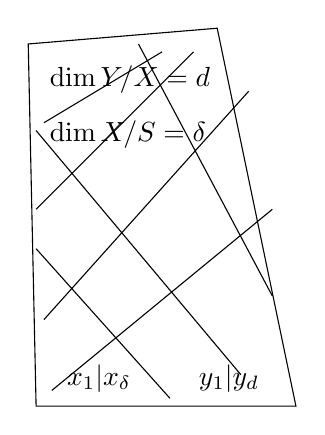
\begin{tikzpicture}[x=1cm,y=1cm]
\draw (0,4.6)--(2.4,4.8)--(3.4,0)--(0.1,0)--cycle;
\node[anchor=west] at (.15,4.15) {$\dim Y/X=d$};
\node[anchor=west] at (.15,3.45) {$\dim X/S=\delta$};
\node at (.9,.35) {$x_1\text{—}x_\delta$};\node at (2.55,.35) {$y_1\text{—}y_d$};
\draw (.2,3.6)--(1.7,4.5) (.1,2.5)--(2.1,4.5) (.2,1.1)--(2.8,4) (.3,.2)--(3.1,2.5) (.1,3.5)--(2.7,.4) (.1,2)--(1.8,.1) (1.4,4.6)--(3.1,1.4);
\end{tikzpicture}}}}

\uline{\S1} Descente \inserted{d'objets plats} par morphismes quelconques

\uline{\S2} Descente d'objets quelconques par morphismes plats.
\margin{\unsure{intervertir}}

\uline{\S3} Application \inserted{de \S1} aux morphismes non ramifiés

\uline{\S4} Cas particuliers élémentaires : Espaces $X/G$, descente galoisienne non ramifiée, le \uline{contre-exemple de Nagata}. Interprétation de la descente plate finie par \uline{opérateurs quasi-différentiels}. Cas de Cartier.
\margin{\uline{\unsure{Conditions de descente}} \uline{\unsure{d'une famille}} \unsure{de schémas} \uline{\unsure{projectifs ?}} \uline{Pas ici le lieu !}}
\margin{\unsure{Les théorèmes|Les résultats} \unsure{vus au} \S1 \unsure{ne sont pas utilisés au} \S\unsure{7}.}
\margin{\S\unsure{1|5} à 7}

\uline{\S5} $\underline{\operatorname{Hom}}_S(X,Y)$ et $f_*(X)$ : formalisme général, cas d'existence pour $X$ fini et plat sur $S$. [Est lié à la \unsure{technique|théorie} de la descente \deleted{seulement} par deux endroits

a) Existence de \uline{Hom} si $X\to S$ est \unsure{géom. injectif|géom. projectif} -- fini et plat --

b) Relations entre l'existence de $f_*(X)$, $\underline{\operatorname{Hom}}_S(X,Y)$, et la possibilité de descente.] Cas particuliers : $\unsure{\check V(\underline F)|\check V(\mathcal F)}$ etc.
\margin{\unsure{Propriétés diverses de permanence}}

\uline{\S6} Application des schémas \uline{Hom} : la géométrie différentielle, les Picard, Greenberg d'égale caractéristique etc

\uline{\S7} \unsure{Hyperproblèmes|Hyperschémas} sur $S$. Critères de représentabilité.

[y inclure aussi le critère général d'existence par théorie des modules formelle]
\margin{\uline{ailleurs ?} Ne vient ici que par l'utilisation dans \unsure{ce qui suit} de l'existence de $\unsure{f_*}$. Pourrait venir \unsure{entièrement} dans Ch. \uline{IV}, mais \unsure{obligerait} d'y développer \unsure{longuement} des \uline{Hom}.}

\uline{\S8} \unsure{4} \deleted{\unsure{Cas particuliers}} \inserted{Théorèmes} \uline{fondamentaux d'existence}

A) Théorie formelle des modules. Extension des solutions\ldots

\uline{\S9} \deleted{B) \unsure{2}} $f_*(X)$ si $X$ est projectif sur $Y$, $Y$ plat et propre sur $S$.

\uline{\S10} C) Picard.
\margin{\unsure{ensemble ?}}

[Critères de simplicité, de propreté, de platitude ?]
% archive foliation: 36
